\begin{homeworkProblem}

Generate uniform distributions over the following geometric objects: \\
(a) Ellipse $(a=2, b=1)$:
$$E_2(a, b)=\left\{(x, y) \in \mathbb{R}^2:\left(\frac{x}{a}\right)^2+\left(\frac{y}{b}\right)^2 \leq 1\right\}$$

(b) Sphere $(r=1)$:
$$S_2(r)=\left\{(x, y, z) \in \mathbb{R}^3: x^2+y^2+z^2=r^2\right\}$$

(c) Ball $(r=1)$:
$$B_3(r)=\left\{(x, y, z) \in \mathbb{R}^3: x^2+y^2+z^2 \leq r^2\right\}$$

(d) Torus $\left(r_0=2, r=1\right)$:
$$T_2\left(r_0, r\right)=\left\{(x, y, z) \in \mathbb{R}^3:\left(r_0-\sqrt{x^2+y^2}\right)^2+z^2=r^2\right\}$$

\solution

(a) 1. Acceptance-Rejection method: \\
\begin{figure}[h]
    \centering
    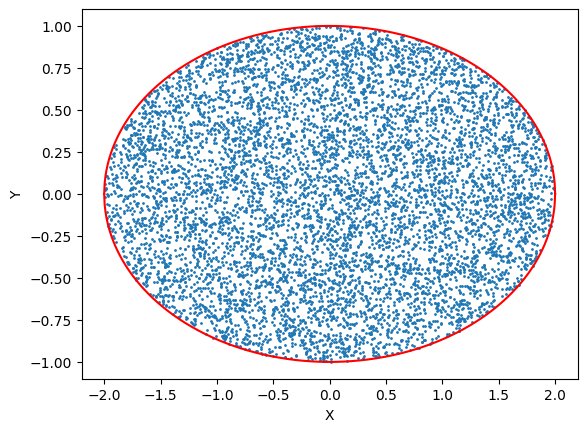
\includegraphics[width=0.8\textwidth]{./figure/p7/a_accept_reject.png}
    \caption{Ellipse sample by Acceptance-Rejection method}
\end{figure}

2. Change of variable: \\
Let $x=a\cdot r\cos\theta$, $y=b\cdot r\sin\theta$, where $\theta\in [0, 2\pi], r\in [0, 1]$. The Jacobian is $|J|=\left|\dfrac{\partial(x, y)}{\partial(r, \theta)}\right|=abr$.

Since the area of the ellipse is $\pi ab$, so the PDF of the ellipse is $f_{X, Y}(x, y)=\dfrac{1}{\pi ab}$. Thus we have
$$f_{R, \Theta}(r, \theta)=f_{X, Y}(x, y)\cdot|J|=\dfrac{1}{\pi ab}\cdot abr=\dfrac{r}{\pi}=f_R(r)f_{\Theta}(\theta)$$
So $R$ and $\Theta$ are independent variables, we can sample them respectively.
\begin{align*}
f_R(r) &= \int_{0}^{2\pi}f_{R, \Theta}(r, \theta)d\theta = 2r \\
F_R(r) &= \int_{0}^{r}f_R(r)dr = r^2 \\
F^{-1}_R(u) &= \sqrt{u} \\
f_{\Theta}(\theta) &= \int_{0}^{1}f_{R, \Theta}(r, \theta)dr = \dfrac{1}{2\pi} \\
F_{\Theta}(\theta) &= \int_{0}^{\theta}f_{\Theta}(\theta)d\theta = \dfrac{\theta}{2\pi} \\
F^{-1}_{\Theta}(u) &= 2\pi u
\end{align*}

$U_1, U_2\stackrel{i.i.d.}{\sim} \Unif(0, 1)$, then let
$$r\leftarrow \sqrt{U_1}, \theta\leftarrow 2\pi U_2$$
Then $(X, Y)$ can be uniformly sampled from the ellipse.
$x = a\cdot r\cos\theta = 2\sqrt{U_1}\cos(2\pi U_2)$, $y = b\cdot r\sin\theta = \sqrt{U_1}\sin(2\pi U_2)$
\begin{figure}[h]
    \centering
    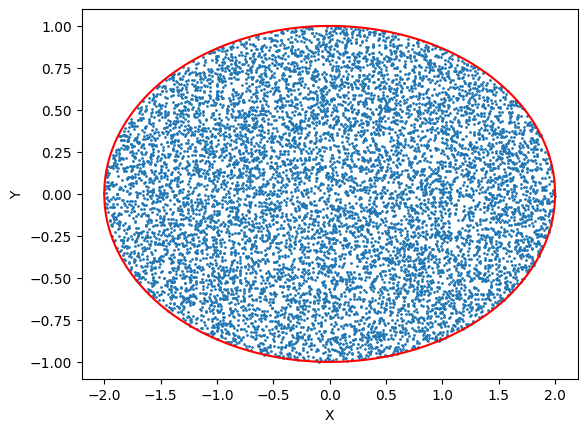
\includegraphics[width=0.8\textwidth]{./figure/p7/a_change_variable.png}
    \caption{Ellipse sample by Change of variable}
\end{figure}


(b) Let $x=r\sin\theta\cos\phi$, $y=r\sin\theta\sin\phi$, $z=r\cos\theta$, where $\theta\in [0, \pi], \phi\in [0, 2\pi]$. The Jacobian is $J=\dfrac{\partial(x, y, z)}{\partial(\theta, \phi)}=\begin{pmatrix}
r\cos\theta\cos\phi & -r\sin\theta\sin\phi \\
r\cos\theta\sin\phi & r\sin\theta\cos\phi \\
-r\sin\theta & 0
\end{pmatrix}$
The Gram matrix $G=J^{\top}J=\begin{pmatrix}
r^2 & 0 \\
0 & r^2\sin^2\theta
\end{pmatrix}$.
The area of the sphere is $4\pi r^2$, so the PDF of the sphere is $f_{X, Y, Z}(x, y, z)=\dfrac{1}{4\pi r^2}$.
So we have
$$f_{\Theta, \Phi}(\theta, \phi) = f_{X, Y, Z}(x, y, z)\cdot|\sqrt{\det(G)}|=\dfrac{1}{4\pi r^2}\cdot r^2\sin\theta = \dfrac{1}{4\pi}\sin\theta=f_{\Theta}(\theta)f_{\Phi}(\phi)$$
So $\Theta$ and $\Phi$ are independent variables, we can sample them respectively.
\begin{align*}
f_{\Theta}(\theta) &= \int_{0}^{2\pi}f_{\Theta, \Phi}(\theta, \phi)d\phi = \dfrac{1}{2}\sin\theta \\
F_{\Theta}(\theta) &= \int_{0}^{\theta}f_{\Theta}(\theta)d\theta = \dfrac{1-\cos\theta}{2} \\
F^{-1}_{\Theta}(u) &= \arccos(1-2u) \\
f_{\Phi}(\phi) &= \int_{0}^{\pi}f_{\Theta, \Phi}(\theta, \phi)d\theta = \dfrac{1}{2\pi} \\
F_{\Phi}(\phi) &= \int_{0}^{\phi}f_{\Phi}(\phi)d\phi = \dfrac{\phi}{2\pi} \\
F^{-1}_{\Phi}(u) &= 2\pi u
\end{align*}

Sample $U_1, U_2\stackrel{i.i.d.}{\sim} \Unif(0, 1)$, then let
$$\theta\leftarrow \arccos(1-2U_1), \phi\leftarrow 2\pi U_2$$
Since $\cos\theta = 1 - 2U_1$, and $\theta\in [0, \pi]$, so $\sin\theta = 2\sqrt{U_1(1-U_1)}$. Then we set that
$$x\gets r\sin\theta\cos\phi = 2\sqrt{U_1(1-U_1)}\cos(2\pi U_2), y\gets r\sin\theta\sin\phi = 2\sqrt{U_1(1-U_1)}\sin(2\pi U_2), z\gets r\cos\theta = 1-2U_1$$
Then $(X, Y, Z)$ can be uniformly sampled from the sphere.

\begin{figure}[ht]
    \centering
    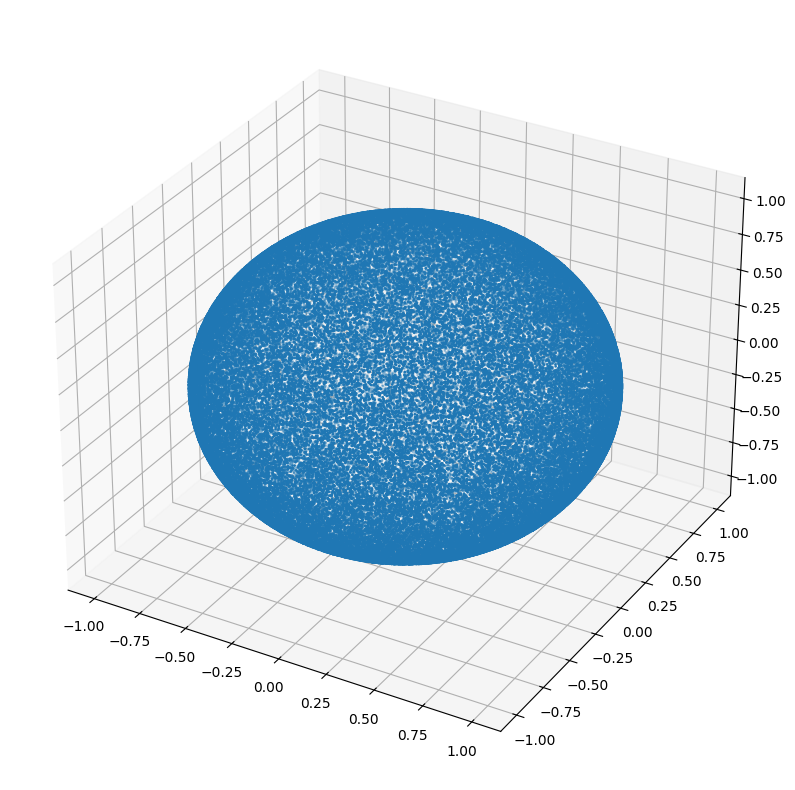
\includegraphics[width=0.48\textwidth]{./figure/p7/b_sample.png}
    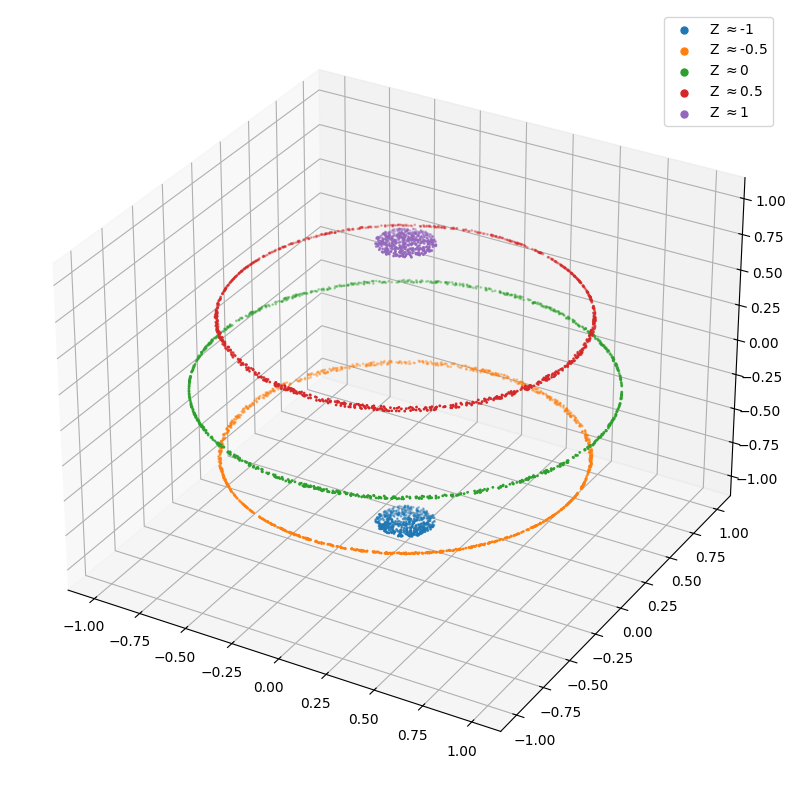
\includegraphics[width=0.48\textwidth]{./figure/p7/b_contour.png}
    \caption{Left: Sphere's sample points. Right: Some contours of the Sphere to show the inner details.}
\end{figure}


(c) Let $x=r\sin\theta\cos\phi$, $y=r\sin\theta\sin\phi$, $z=r\cos\theta$, where $\theta\in [0, \pi], \phi\in [0, 2\pi], r\in [0, 1]$. The Jacobian is $J=\dfrac{\partial(x, y, z)}{\partial(r, \theta, \phi)}=r^2\sin\theta$.

Since the volume of the ball is $\dfrac{4}{3}\pi r^3=\dfrac{4}{3}\pi$, so the PDF of the ball is $f_{X, Y, Z}(x, y, z)=\dfrac{3}{4\pi}$. Thus we have
$$f_{R, \Theta, \Phi}(r, \theta, \phi)=f_{X, Y, Z}(x, y, z)\cdot|J|=\dfrac{3}{4\pi}\cdot r^2\sin\theta=f_R(r)f_{\Theta}(\theta)f_{\Phi}(\phi)$$
So $R$, $\Theta$ and $\Phi$ are independent variables, we can sample them respectively.

\begin{align*}
f_R(r) &= \int_{0}^{2\pi}\int_{0}^{\pi}f_{R, \Theta, \Phi}(r, \theta, \phi)d\theta d\phi = 3r^2 \\
F_R(r) &= \int_{0}^{r}f_R(r)dr = r^3 \\
f_{\Theta}(\theta) &= \int_{0}^{2\pi}\int_{0}^{1}f_{R, \Theta, \Phi}(r, \theta, \phi)dr d\phi = \dfrac{1}{2}\sin\theta \\
F_{\Theta}(\theta) &= \int_{0}^{\theta}f_{\Theta}(\theta)d\theta = \dfrac{1}{2}(1-\cos\theta) \\
f_{\Phi}(\phi) &= \int_{0}^{2\pi}\int_{0}^{1}f_{R, \Theta, \Phi}(r, \theta, \phi)dr d\theta = \dfrac{1}{2\pi} \\
F_{\Phi}(\phi) &= \int_{0}^{\phi}f_{\Phi}(\phi)d\phi = \dfrac{\phi}{2\pi}
\end{align*}

$U_1, U_2, U_3\stackrel{i.i.d.}{\sim} \Unif(0, 1)$, then let
$$r\leftarrow \sqrt[3]{U_1}, \theta\leftarrow \arccos(1-2U_2), \phi\leftarrow 2\pi U_3$$
We can ree-write $\cos\theta=1-2U_2$, and $\sin\theta=2\sqrt{U_2(1-U_2)}$ to save computational complexity.
Then $(X, Y, Z)$ can be uniformly sampled from the ball.

\begin{figure}[ht]
    \centering
    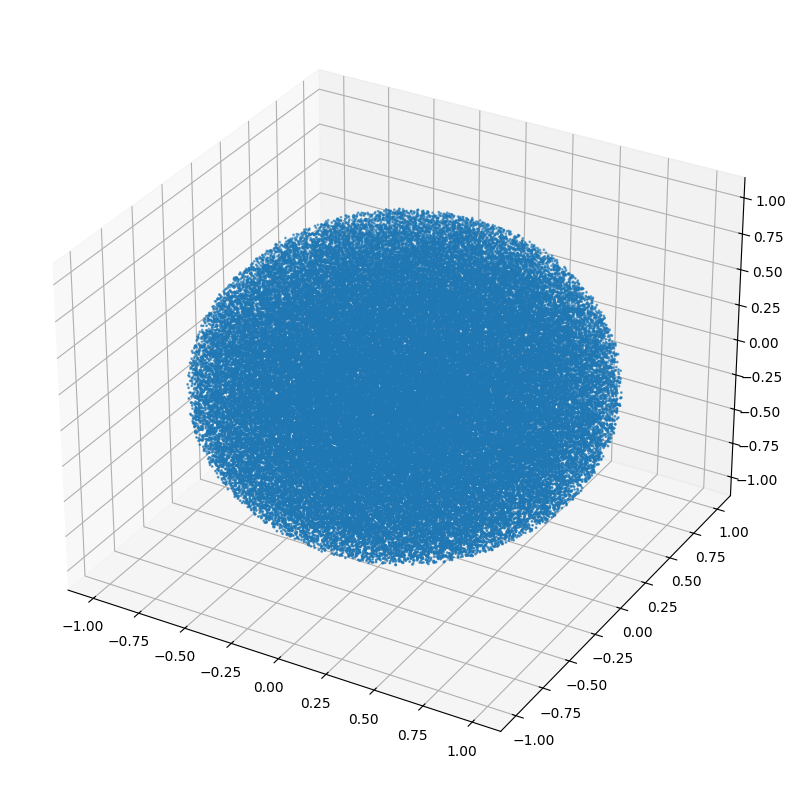
\includegraphics[width=0.48\textwidth]{./figure/p7/c_sample.png}
    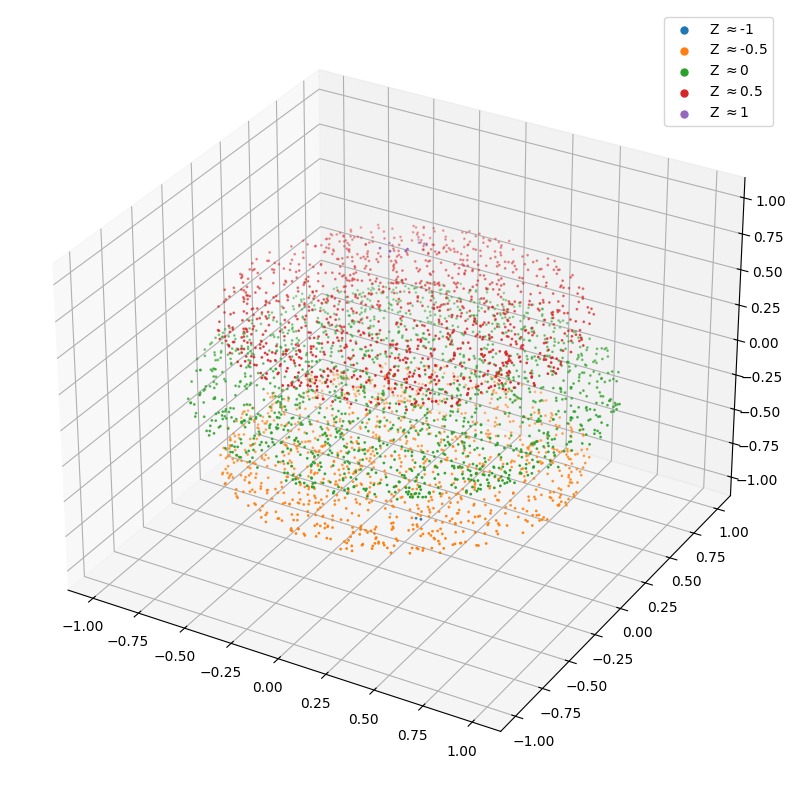
\includegraphics[width=0.48\textwidth]{./figure/p7/c_contour.png}
    \caption{Left: Ball's sample points. Right: Some contours of the Ball to show the inner details.}
\end{figure}


(d) Let $x=(r_0+r\cos\theta)\cos\phi, y=(r_0+r\cos\theta)\sin\phi, z=r\sin\theta$, where $\theta\in [0, 2\pi], \phi\in [0, 2\pi], r\in [0, 1]$. The Jacobian is $J=\dfrac{\partial(x, y, z)}{\partial(r, \theta, \phi)}=\begin{pmatrix}
-r\sin\theta\cos\phi & -(r_0+r\cos\theta)\sin\phi \\
-r\sin\theta\sin\phi & (r_0+r\cos\theta)\cos\phi \\
r\cos\theta & 0
\end{pmatrix}$.
So the Gram matrix $G=J^{\top}J=\begin{pmatrix}
r^2 & 0 \\
0 & (r_0+r\cos\theta)^2
\end{pmatrix}$.
Since $r=1$, so $r\cos\theta>0$

$$\dS = \sqrt{\det(G)}\dtheta\dphi = r(r_0+r\cos\theta)\dr\dtheta\dphi$$
\begin{align*}
S &= \oint \dS \\
&= \int_{0}^{2\pi}\int_{0}^{2\pi}r(r_0+r\cos\theta)d\theta d\phi \\
&= 4\pi^2r\cdot r_0 \\
&= 8\pi^2
\end{align*}
$f_{X,Y,Z}(x,y,z)=\dfrac{1}{4\pi^2r\cdot r_0}=\dfrac{1}{8\pi^2}$, so
$$f_{\Theta, \Phi}(\theta,\phi)=\dfrac{1}{4\pi^2r_0}\cdot r(r_0+r\cos\theta)=\dfrac{r_0+r\cos\theta}{4\pi^2r_0} = \dfrac{2+\cos\theta}{8\pi^2}=f_{\Theta}(\theta)f_{\Phi}(\phi)$$
So $\Theta$ and $\Phi$ are independent variables, we can sample them respectively.

\begin{align*}
f_{\Theta}(\theta) &= \int_{0}^{2\pi}f_{\Theta, \Phi}(\theta,\phi)d\phi = \dfrac{r_0+r\cos\theta}{2\pi r_0} = \dfrac{2+\cos\theta}{4\pi} \\
F_{\Theta}(\theta) &= \int_{0}^{\theta}f_{\Theta}(\theta)d\theta = \dfrac{1}{2\pi}\theta + \dfrac{r}{2\pi r_0}\sin\theta = \dfrac{1}{2\pi}\theta + \dfrac{1}{4\pi}\sin\theta \\
f_{\Phi}(\phi) &= \int_{0}^{2\pi}f_{\Theta, \Phi}(\theta,\phi)d\theta = \dfrac{1}{2\pi} \\
F_{\Phi}(\phi) &= \int_{0}^{\phi}f_{\Phi}(\phi)d\phi = \dfrac{\phi}{2\pi}
\end{align*}

$U_1, U_2\stackrel{i.i.d.}{\sim} \Unif(0, 1)$, then let
$\theta$ be the solution that $\dfrac{1}{2\pi}\theta + \dfrac{1}{4\pi}\sin\theta=U_1$, $\phi\leftarrow 2\pi U_2$. $\theta$ has no closed form solution, but we can use the toolkits to solve the equation as the valid CDF must exist a solution.

Then $(X, Y, Z)$ can be uniformly sampled from the Torus whose $r_0=2,r=1$.

\begin{figure}[ht]
    \centering
    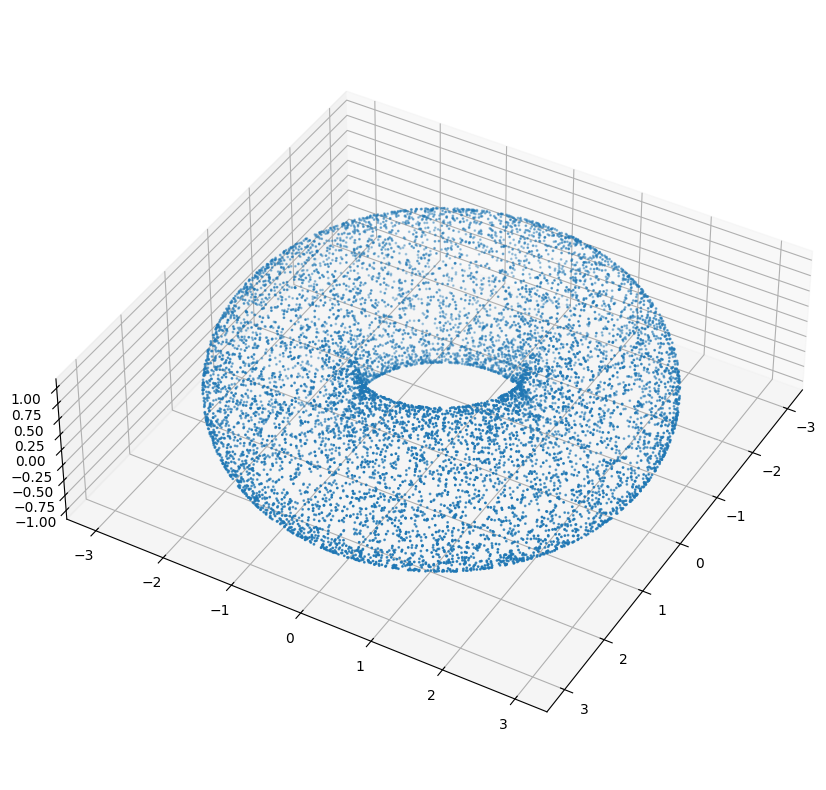
\includegraphics[width=0.48\textwidth]{./figure/p7/d_sample.png}
    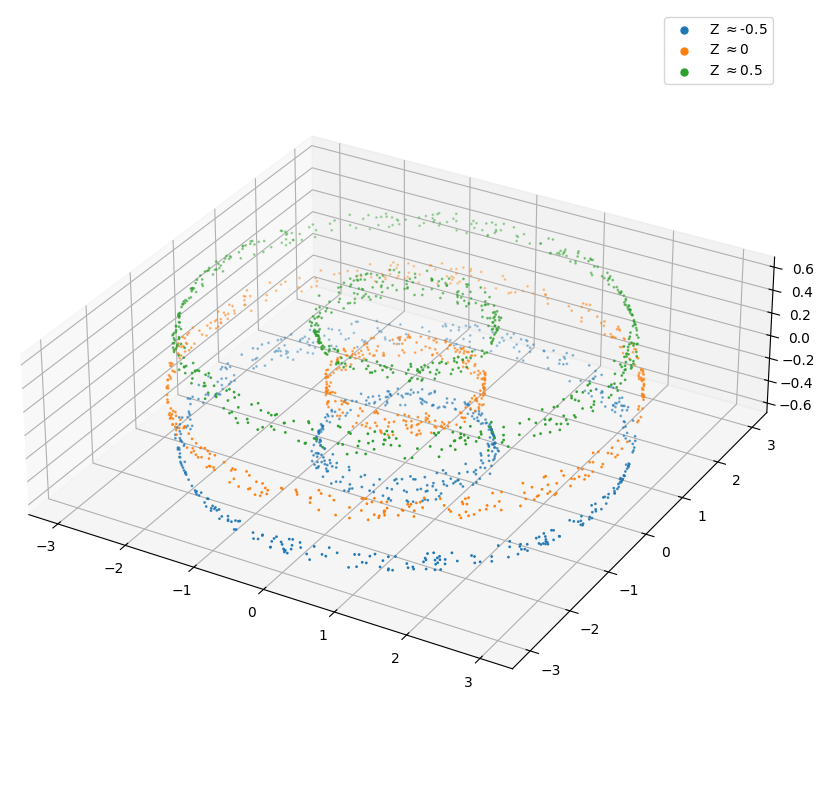
\includegraphics[width=0.48\textwidth]{./figure/p7/d_contour.png}
    \caption{Left: Torus's sample points. Right: Some contours of the Torus to show the inner details.}
\end{figure}

\end{homeworkProblem}

\newpage